\documentclass[main.tex]{subfiles}
\begin{document}
\chapter{Bonus: (Co)algebras and (Co)induction}\label{chap:coalgebra}
%TODO: bisimulation of DFA is equality of languages.
\section{(Co)algebras and (Co)induction}

In this section, we will introduce (co)algebras and (co)induction and ask you to fill out some gaps. While the definitions are given for an arbitrary category $\mathbf{C}$, all of the examples and exercises will be done on \textbf{Set}.

\subsection{Algebras}
The term \textit{algebra} has a few different meanings and here we will more precisely consider $F$--algebras for some endofuntor $F:\mathbf{C}\rightsquigarrow \mathbf{C}$. Nevertheless, all the objects that are referred to as algebras have a common motto: \textit{algebras only care about structure}.

For instance, in a first year algebra course, groups are studied up to isomorphisms (maps that preserve the structure) because all the useful properties of a group are determined completely by how the operation acts on the underlying set. As a concrete example, the groups $\Z_2 \times \Z_3$ and $\Z_6$ are the same group even if their elements have different names. It is a similar situation for rings, vector spaces and a lot more mathematical objects.

Before giving the general definition of an $F$--algebra, we categorify the definition of a group.
\begin{exmp}\label{exmpgroup}
	Usually, a group is defined as a set $G$ along with an operation $\cdot: G\times G\rightarrow G$ satisfying some conditions, namely, associativity, existence of an identity and existence of an inverse for each element. It is then a formal consequence that the identity and inverses are unique.
	
	Therefore, it is equivalent to define a group as a set $G$ with a binary operation $\cdot$, an identity $1 \in G$ and an inverse $g^{-1}$ for all $g \in G$ that satisfy some properties. In order to abide to the categorical mindset, it is better to view the identity as a morphism $1: \mathbf{1} \rightarrow G$ ($\mathbf{1}$ is the final object, i.e.: a singleton) and describe inverses with a morphism $(-)^{-1} : G \rightarrow G$. A few additional diagrams have to commute for $G$ to satisfy all axioms of a group, but we leave their construction as an exercise. We conclude that a group can be seen as a morphism \[[1,(-)^{-1}, \cdot] : \mathbf{1} + G + (G\times G) \rightarrow G.\]
	This is our first example of an $F$--algebra, here $F:\textbf{Set}\rightsquigarrow \textbf{Set}$ sends a set $G$ to $\mathbf{1}+G+(G\times G)$ and a morphism $f$ to $[\id_{\mathbf{1}}, f, (f,f)]$.
	
	Note that since we have not used the fact that $G$ is a set, this definition gives rise to groups in other categories than \textbf{Set} provided they have a final object, products and coproducts.
\end{exmp}
\begin{exer}[1pt]
    Draw the additional diagrams that $G$, $\cdot$, $1$ and $(-)^{-1}$ should satisfy to obtain a group.
\end{exer}
\begin{defn}[$F$--algebra]
    Let $F:\mathbf{C}\rightsquigarrow \mathbf{C}$ be a functor, an $F$--\textbf{algebra} is an object $A \in \mathbf{C}_0$ along with a morphism $\alpha: F(A) \rightarrow A \in \mathbf{C}_1$ called the \textbf{structure map}.
\end{defn}
\begin{exmps}
	\begin{enumerate}
		\item[]
		\item Since a monoid $M$ only has a binary operation and an identity, it can be represented as an algebra $[1,\cdot] : \mathbf{1} + (M\times M) \rightarrow M$. Similarly, one can construct algebras that represent rings and vector spaces, but not fields (why?).
		\item We will see later that the induction principle we know comes from the algebra $[0,\succ]: \mathbf{1} + \N \rightarrow \N$, where $0(\ast) = 0$ and $\succ(n) = n+1$.
		\item Although we will not use them often, there are algebras in different categories than \textbf{Set}. In computer science, we often use induction to reason about lists, we will see that this is because lists are algebras. More precisely, for a type $A$, the type $A^*$ of lists with elements of type $A$ is has an algebra structure $[\textsf{nil}, \textsf{cons}]: 1+ (A\times A^*) \rightarrow A^*$ given by $\textsf{nil}(*) = \varepsilon \in A^*$ (the empty list) and $\textsf{cons}(a, w) = w\cdot a \in A^*$ (concatenation). The category in which this algebra lives depends on the programming language and types considered.
	\end{enumerate}
\end{exmps}
\begin{rem}
	The components of the structure map (i.e.: $0$ and $\succ$ in the second example) are often called the \textbf{constructors} because they define rules to construct elements of the algebra using other elements as building blocks.
\end{rem}
As you might expect $F$--algebras form a category, denoted $\text{Alg}(F)$, with the following notion of morphism.
\begin{defn}[$F$--algebra homomorphism]\label{alghom}
	Let $F:\mathbf{C}\rightsquigarrow \mathbf{C}$ be a functor and $\alpha: F(A) \rightarrow A$ and $\beta:F(B) \rightarrow B$ be $F$--algebras. An $F$--\textbf{algebra homomorphism} from the former to the latter is a morphism $f:A\rightarrow B$ that makes this square commute.
	\begin{equation}\label{diag-alghom}
		\begin{tikzcd}
			F(A) \arrow[d, "\alpha"'] \arrow[r, "F(f)"] & F(B) \arrow[d, "\beta"] \\
			A \arrow[r, "f"']                           & B                       
		\end{tikzcd}
	\end{equation}
	This definition also clarifies why we require $F$ to be a functor.
\end{defn}
\begin{exmp}
	Let $F = X \mapsto \mathbf{1} + X + (X\times X)$ be the functor discussed Example \ref{exmpgroup}. An $F$--algebra homomorphism is represented by the following square.
	\begin{equation}\label{diag-homgroup}
		\centering
		\begin{tikzcd}
			\mathbf{1}+G+(G\times G) \arrow[d, "{[1_G,(-)^{-1},\cdot]}"'] \arrow[r, "{[\id_{\mathbf{1}},f,(f,f)]}"] & \ \mathbf{1}+H+(H\times H) \arrow[d, "{[1_H,(-)^{-1}, \cdot]}"] \\
			G \arrow[r, "f"']                           & H                       
		\end{tikzcd}
	\end{equation}
	Unwrapped, this says that $f(1_G) = 1_H$, $f(g^{-1}) = f(g)^{-1}$ and $f(g\cdot g') = f(g)\cdot f(g')$ for all $g,g' \in G$, i.e.: if both algebras represent groups as seen in Example \ref{exmpgroup}, it is a group homomorphism.
\end{exmp}
\subsection{Coalgebras}
Now that we have a categorical notion of algebra, we can look at its dual.
\begin{defn}[$F$--coalgebra]
	Let $F:\mathbf{C}\rightsquigarrow \mathbf{C}$ be a functor, an $F$--\textbf{coalgebra} is an object $A \in \mathbf{C}_0$ called the \textbf{carrier} along with a morphism $\omega: A\rightarrow F(A)$ called the \textbf{behavior map}. We will refer to a coalgebra with $A$, $\omega$ or the pair $(A, \omega)$.
\end{defn}
\begin{exmps}\label{exmpcoalg}
	\begin{enumerate}
		\item If $F$ is the identity on \textbf{Set}, then an $F$--coalgebra is just an endomorphism $\omega:A\rightarrow A$ and it is sometimes called a \textbf{dynamical system}. You can think of the elements of $A$ as states and $\omega$ as the transition map for the system.
        \item Let $\Str_{\N}:\textbf{Set}\rightsquigarrow\textbf{Set} = \N \times (-)$ be the functor sending a set $X$ to $\N\times X$ and a function $f: X\rightarrow Y$ to $\id_{\N} \times f : \N\times X \rightarrow \N\times Y$. An example of a $\Str_{\N}$--coalgebra is the set $\N^{\N}$ of all infinite sequences (also called \textbf{streams}) of natural numbers with the structure map $(\head,\tail): \N^{\N} \rightarrow \N \times \N^{\N}$ given by \[\head:\N^{\N} \rightarrow \N = \sigma \mapsto \sigma(0)\quad \text{ and } \quad \tail:\N^{\N} \rightarrow \N^{\N} = \sigma \mapsto \sigma \circ \succ.\]
        Unsurprisingly, we call $\head(\sigma)$ and $\tail(\sigma)$ the \textbf{head} and \textbf{tail} of the stream $\sigma$ respectively.
	\end{enumerate}
\end{exmps}
\begin{exer}[1pt]
    Denoting $2 = \{0,1\}$, let $F = 2\times (-)^A$ send a set $X$ to $2 \times X^A$ and a function $f: X \rightarrow Y$ to $\id_2 \times (f \circ -): 2\times X^A \rightarrow 2 \times Y^A$. When $A$ is finite, show that there is a correspondence between $F$--coalgebras with a finite carrier and DFAs over the alphabet $A$ without initial states.
\end{exer}
\begin{rem}
	The components of the behavior map (i.e.: $h$ and $t$ in the second example) are often called \textbf{destructors} or \textbf{observers} because they decompose elements of the coalgebra.
\end{rem}
We define morphisms of $F$--coalgebras in order to obtain a category $\text{Coalg}(F)$.
\begin{defn}[$F$--coalgebra homomorphism]
	Let $F:\mathbf{C}\rightsquigarrow \mathbf{C}$ be a functor and $\alpha: A \rightarrow F(A)$ and $\beta:B \rightarrow F(B)$ be $F$--coalgebras. An $F$--\textbf{coalgebra homomorphism} from the former to the latter is a morphism $f:A\rightarrow B \in \mathbf{C}_1$ that makes \eqref{diag-coalghom} commute.
	\begin{equation}\label{diag-coalghom}
		\centering
		\begin{tikzcd}
			A \arrow[r, "f"] \arrow[d, "\alpha"'] & B \arrow[d, "\beta"] \\
			F(A) \arrow[r, "F(f)"']               & F(B)                
		\end{tikzcd}
	\end{equation}
\end{defn}

\subsection{Induction}
Induction is a very well known and prevalent proof principle. In it most common form, it says that for any predicate $P$ on $\N$, if $P(0)$ is true and $P(n) \implies P(n+1)$ is true for any $n \in \N$, then so is $P(n)$ for any $n\in \N$. In this section, we use the power of algebras to generalize this proof principle and give a few examples.

\begin{defn}[Initial algebra]\label{initalg}
	Let $F:\mathbf{C}\rightsquigarrow \mathbf{C}$ be a functor, an \textbf{initial algebra} is an initial object in the category of $F$--algebras. Namely, it is an algbera $(A, \alpha)$ such that for any other algebra $(B, \beta)$, there is a unique $f : A\rightarrow B$ making the following square commute.
	\begin{equation}\label{diag-initalg}
		\centering
		\begin{tikzcd}
			F(A) \arrow[d, "\alpha"'] \arrow[r, dashed, "F(f)"] & F(B) \arrow[d, "\beta"] \\
			A \arrow[r, dashed, "f"']                           & B                       
		\end{tikzcd}
	\end{equation}
\end{defn}
\begin{exmp}
    The algebra $(\N, [0,\succ])$ is initial for the functor $\mathbf{1} + (-)$. Indeed, let $[z,s]:\mathbf{1}+X \rightarrow X$ be another algebra for this functor, then a map $f:\N\rightarrow X$ that makes the following diagram commute must necessarily satisfy $f(0) = z(\ast)$ and $f(n) = s^n(z(\ast))$.
    \begin{equation}\label{diag-initN}
        \centering
        \begin{tikzcd}
            \mathbf{1}+\N \arrow[d, "{[0,\succ]}"'] \arrow[r, "{[\id_{\mathbf{1}}, f]}"] & \mathbf{1}+X \arrow[d, "{[z,s]}"] \\
            \N \arrow[r, "f"']                           & X                       
        \end{tikzcd}
    \end{equation}
    This completely determines $f$ and moreover, defining $f$ like this for any ($\mathbf{1} + (-)$)-algebra $(X,[z,s])$ yields an algebra homomorphism. 
\end{exmp}
\begin{exer}[2pts]\label{exer-initAlg}
    Show that the algebra for lists $[\textsf{nil}, \textsf{cons}]: 1 + A \times A^* \rightarrow A^*$ is initial for the functor $1+A \times (-): \textbf{Set}\rightsquigarrow \textbf{Set}$ (you know its action on sets, on morphisms it sends $f:X \rightarrow Y$ to $[\id_{\mathbf{1}}, (\id_A, f)]$).
\end{exer}
We already know that initial objects are unique up to unique isomorphisms, but Lambek also showed furthermore that initial $F$--algebras are fixed points of $F$.
\begin{prop}[Lambek]\label{initialiso}
	Let $F:\mathbf{C}\rightsquigarrow \mathbf{C}$, if $(A,\alpha)$ is an initial $F$--algebra, then $\alpha:F(A)\rightarrow A$ is an isomorphism.
\end{prop}
\begin{exer}[1.5pts]
    Prove Proposition \ref{initialiso}. \textbf{Hint:} Consider the algebra $F(\alpha): F^2(A) \rightarrow F(A)$.
\end{exer}

Initial algebras generalize the inductive reasoning we use with the natural numbers to much more settings. We distinguish two cases where induction is used: inductive definitions and the induction proof principle. 

For the former, the general idea is that, given an initial $F$--algebra $(A,\alpha)$, we can easily define a function $f:A\rightarrow B$ by looking at how it acts on constructors. Indeed, with only this data, we can construct an $F$--algebra structure on $B$ such that the unique homomorphism $!:A\rightarrow B$ acts exactly like $f$.
\begin{exmp}[Inductive definition]
	Recall that $(A^*, [\textsf{nil}, \textsf{cons}])$ is the initial ($1+A\times(-)$)-algebra. We would like to define the function $\textsf{len}:A^* \rightarrow \N$ that computes the length of a list. Intuitively, it satisfies the equations \[\textsf{len}(\textsf{nil}) = 0 \quad \quad \textsf{len}(\textsf{cons}(a,l)) = 1+\textsf{len}(l).\]
	Then, if we construct the ($1+A\times(-)$)-algebra $[z, s]:1+ A\times \N \rightarrow \N$ defined by $z(\ast) = 0$ and $s(a,n) = 1+n$, we can verify that the unique algebra homomorphism $!:A^*\rightarrow \N$ is the function $\textsf{len}$ because both make the following diagram commute.
	\begin{equation}\label{diag-lendef}
	\centering
		\begin{tikzcd}
			1+A\times A^* \arrow[d, "{[\textsf{nil}, \textsf{cons}]}"'] \arrow[r, "1+\text{id}_A\times !"] & 1+A\times \N \arrow[d, "{[z,s]}"] \\
			A^* \arrow[r, "!=\textsf{len}"']                                                                            & \N                               
		\end{tikzcd}
	\end{equation}
\end{exmp}
\begin{exer}[1pt]
    Use the initiality of $\N$ for the functor $1+(-)$ to define the function $n \mapsto 2^n$.
\end{exer}
Generalizing proofs by induction in this context is more involved and we will need the definition of $F$--congruences. While $F$--algebra homomorphisms are maps between algebras that preserve the structure, an $F$--congruence is a relation between two algebras that preserves the structure.

\begin{defn}
	Let $F:\mathbf{C}\rightsquigarrow \mathbf{C}$ be a functor and $(A,\alpha)$ and $(B, \beta)$ be $F$--algebras, a relation $R \subseteq A \times B$ is an $F$\textbf{-congruence} if there is a structure map $\gamma:F(R) \rightarrow R$ such that the projections $\pi_1:R\rightarrow A$ and $\pi_2:R \rightarrow B$ are algebra homomorphisms making this diagram commute.
	\begin{equation}\label{diag-congruence}
		\centering
		\begin{tikzcd}
			F(A) \arrow[d, "\alpha"'] & F(R) \arrow[d, "\gamma"] \arrow[l, "F\pi_1"'] \arrow[r, "F\pi_2"] & F(B) \arrow[d, "\beta"] \\
			A                         & R \arrow[r, "\pi_2"'] \arrow[l, "\pi_1"]                          & B                      
		\end{tikzcd}
	\end{equation}
\end{defn}
\begin{exmp}
	If $F$ is the identity functor, then for any algebras $(A, \alpha)$ and $(B, \beta)$ and any relation $R \subseteq A\times B$, $\gamma = (\alpha \circ \pi_1, \beta \circ \pi_2)$ is a structure map making $R$ into an $F$--congruence.
\end{exmp}
\begin{exer}[2pts]
    Let $F = \mathbf{1} + (-)$, we have already seen that $\N$ is an initial $F$--algebra.
    \begin{enumerate}[(a)]
        \item Give a necessary and sufficient condition for $R \subseteq \N \times \N$ to be an $F$--congruence.
        \item Conclude that for any $F$--congruence $R \subseteq \N\times \N$, $\forall n \in \N, (n,n) \in \R$.
    \end{enumerate}
\end{exer}
The next theorem generalizes the previous exercise.
\begin{thm}[General induction]\label{induction} Let $F:\mathbf{C}\rightsquigarrow \mathbf{C}$ be a functor and $(A, \alpha)$ be an initial $F$--algebra, if $R\subseteq A\times A$ is an $F$--congruence, then it is reflexive, that is $(a,a) \in R$ for all $a \in A$.
\end{thm}
\begin{exer}[1.5pts]
    Prove Theorem \ref{induction}.
\end{exer}
\begin{exmp}[Induction in $\N$]
	We will see how the induction principle in Theorem \ref{induction} implies the usual induction principle. Let $P$ be a predicate on $\N$ that satisfies $0 \in P$ and $n\in P \implies n+1 \in P$. One can show that $P\times P \subseteq \N\times \N$ is an $F$--congruence and by general induction, $(n,n) \in P \times P$ for all $n \in \N$, i.e.: $\forall n\in \N, n \in P$.
\end{exmp}
Although going through all these abstractions and definitions seems like a really convoluted way to prove the induction principle, it lead us to two new concepts. First, we can now use inductive reasoning on all sorts of algebras even if they are in no way similar to $\N$. Second, we obtained an easy access to the dual of induction which we present in the following section.

\subsection{Coinduction}
\begin{defn}[Final coalgebra]
	Let $F:\mathbf{C}\rightsquigarrow \mathbf{C}$ be a functor, a \textbf{final coalgebra} is a final object in the category of $F$--coalgebras. Namely, it is a coalgbera $(A, \omega)$ such that for any other coalgebra $(B, \psi)$, there is a unique morphism $f: B\rightarrow A$ making the following square commute.
	\begin{equation}\label{diag-fincoalg}
	\centering
	\begin{tikzcd}
	B \arrow[d, "\psi"'] \arrow[r, dashed, "f"] & A \arrow[d, "\omega"] \\
	F(B) \arrow[r, dashed, "F(f)"']                           & F(A)                       
	\end{tikzcd}
    \end{equation}
    Since final coalgebras are unique up to unique homomorphism, we will refer to \textbf{the} final coalgebra.
\end{defn}
\begin{exmp}\label{exmp-finalcoalgStr}
    The $\Str_{\N}$--coalgebra $(\head,\tail): \N^{\N} \rightarrow \N \times \N^{\N}$ is final. That is, for any $\Str_{\N}$--coalgebra, $(h,t): X \rightarrow \N \times X$, there is unique morphism $!:X \rightarrow \N^{\N}$ making \eqref{diag-finalcoalgStr} commute.
    \begin{equation}\label{diag-finalcoalgStr}
        \begin{tikzcd}
            X \arrow[d, "{(h,t)}"'] \arrow[r, "!", dotted]  & \N^{\N} \arrow[d, "{(\head,\tail)}"] \\
            \N\times X \arrow[r, "\id_N \times !"', dotted] & \N \times \N^{\N}                   
        \end{tikzcd}
    \end{equation}
    The equation corresponding to \eqref{diag-finalcoalgStr} is $(\head, \tail) \circ ! = (\id_{\N} \times !) \circ (h,t)$. We can decompose it into $\head \circ ! = h$ and $\tail \circ ! = ! \circ t$. The first equation tells us that $!(x)$ starts with the number $h(x)$ and the second equation tells us that the tail of $!(x)$ is the stream corresponding to $t(x)$ (via $!$). In short, we have $!(x) = h(x) \cdot !(t(x))$. If we further decompose the tail, we obtain
    \[!(x) = h(x) \cdot h(t(x)) \cdot h(t(t(x))) \cdots h(t^n(x))\cdots.\]
    This should convince you that the only suitable choice for $!$ is $x \mapsto (n \mapsto h(t^n(x)))$.
\end{exmp}
\begin{exer}[3pts]\label{exer-finalcoalg}
	 Let $F = 2\times (-)^A$ with $A$ finite and consider the $F$--coalgebra \[(\varepsilon?, \omega): 2^{A^*} \rightarrow 2\times (2^{A^*})^A,\]
	 where for a language $L \subseteq A^*$ ($\varepsilon$ denotes the empty string), \[\varepsilon?(L) = \begin{cases}1 & \varepsilon \in L\\0 & \text{o/w}\end{cases}, \quad \quad \omega(L) = a \mapsto L_a = \{w \in A^* \mid a \cdot w \in L\}.\] The language $L_a = \omega(L)(a)$ is sometimes called the left $a$--derivative of $L$. Given a DFA $M$ corresponding to the coalgebra $[f,\delta]: Q\rightarrow 2\times Q^A$, show that the function 
	 \[o: Q \rightarrow 2^{A^*} = q\mapsto \{w \in A^* \mid \text{ $M$ accepts $w$ when starting in state $q$}\}\] is the only map making \eqref{diag-finalcoalgexmp} commute. 
    \begin{equation}\label{diag-finalcoalgexmp}
    \centering
    \begin{tikzcd}
        & 2                                                     \\
        X \arrow[d, "\delta"'] \arrow[r, "o", dashed] \arrow[ru, "f"] & 2^{A^*} \arrow[d, "\omega"] \arrow[u, "\varepsilon?"] \\
        X^A \arrow[r, "o^A"', dashed]                               & (2^{A^*})^A                                          
    \end{tikzcd}
    \end{equation}
\end{exer}
\begin{rem}
    Extending your proof to $X$ not necessarily finite, you could obtain the fact that $(2^{A^*}, (\varepsilon?, \omega))$ is the final $2\times (-)^A$ coalgebra.
\end{rem}
\begin{prop}\label{prop-lambek}
    If $\omega: A \rightarrow F(A)$ is a final $F$--coalgebra, then $\omega$ is an isomorphism.
\end{prop}
\begin{exer}[0.5pts]
    Prove Proposition \ref{prop-lambek}.
\end{exer}

Final coalgebras lets us use \textbf{coinductive definitions}. You will see that they are quite similar to inductive definitions you are used to. In fact, as the name suggests, they are dual to each other, but we will not make this formal here.
\begin{exmps}[Coinductive definitions]
	Fix some set $A$ and consider the functor $\Str_A = A \times (-)$, similarly to $\Str_{\N}$, the set $A^{\N}$ of streams in $A$ is the final $\Str_A$--coalgebra with the behavior map $(\head, \tail)$ as defined in Example \ref{exmpcoalg}. We will define three different maps using the finality of $A^{\N}$.
	
	\begin{enumerate}
		\item The function $\sfeven: A^{\N}\rightarrow A^{\N}$ takes a stream $\sigma = (\sigma(0), \sigma(1), \dots)$ and maps it to the stream of elements of $\sigma$ at even positions, namely $\sfeven(\sigma) = (\sigma(0), \sigma(2), \dots )$. To define it coinductively, we need to describe how destructors act on it. It is easy to verify that 
		\[\head(\sfeven(\sigma)) = \head(\sigma) \quad \text{and} \quad \tail(\sfeven(\sigma)) = \sfeven(\tail(\tail(\sigma))).\]
        Hence, if we define a new $\Str_A$--coalgebra on $A^{\N}$ by $(h,t) = (\head, \tail^2 = \tail \circ \tail)$, then we conclude by finality and commutativity of the following diagram that $!:A^{\N} \rightarrow A^{\N}$ is the function $\sfeven$.
		\begin{equation}\label{diag-evendef}
			\centering
			\begin{tikzcd}
				A^{\N} \arrow[d, "{(\head, \tail^2)}"'] \arrow[r, "!", dashed] & A^{\N} \arrow[d, "{(\head, \tail)}"] \\
				A\times A^{\N} \arrow[r, "\text{id}_A \times !"', dashed]      & A\times A^{\N}                      
			\end{tikzcd}
		\end{equation}
		\item The operation of merging two streams is described by the function $\sfmerge: A^{\N} \times A^{\N} \rightarrow A^{\N}$ mapping $(\sigma, \tau)$ to $(\sigma(0), \tau(0), \sigma(1), \tau(1), \dots)$. Observe that destructors act as follows:
		\[\head(\sfmerge(\sigma, \tau)) = \head(\sigma) \quad \text{and} \quad \tail(\sfmerge(\sigma,\tau)) = \sfmerge(\tau, \tail(\sigma)).\]
		The existence of $\sfmerge$ is then proven with finality of $A^{\N}$ and the following coalgebra behavior map (where $\pi_1$ and $\pi_2$ are the projections):
		\[(\head\circ \pi_1, \pi_2, \tail \circ \pi_1): A^{\N} \times A^{\N} \rightarrow A \times A^{\N} \times A^{\N}.\]
	\end{enumerate}
\end{exmps}
\begin{exer}[1pts]
    Similarly to the first item, show that the function $\sfodd: A^{\N}\rightarrow A^{\N}$ mapping $\sigma = (\sigma(0), \sigma(1), \dots)$ to $\sfodd(\sigma) = (\sigma(1), \sigma(3), \dots )$ can be defined coinductively.
\end{exer}

There is also a dual to the induction proof principle for which we need to define bisimulation.
\begin{defn}[$F$--bisimulation]
	Let $F:\mathbf{C}\rightsquigarrow \mathbf{C}$ be a functor and $(A,\omega)$ and $(B, \psi)$ be $F$--coalgebras, a relation $R \subseteq A \times B$ is an $F$\textbf{--bisimulation} if there is a behavior map $\gamma:R \rightarrow F(R)$ such that the projections $\pi_1:R\rightarrow A$ and $\pi_2:R \rightarrow B$ are coalgebra homomorphisms making this diagram commute.
	\begin{equation}\label{diag-mergedef}
		\centering
		\begin{tikzcd}
			A \arrow[d, "\omega"'] & R \arrow[d, "\gamma"] \arrow[l, "\pi_1"'] \arrow[r, "\pi_2"] & B \arrow[d, "\psi"] \\
			F(A)                         & F(R) \arrow[r, "F\pi_2"'] \arrow[l, "F\pi_1"]                          & F(B)                      
		\end{tikzcd}
	\end{equation}
\end{defn}

\begin{thm}[Coinductive proof principle]\label{thm-coind} Let $F:\mathbf{C}\rightsquigarrow \mathbf{C}$ be a functor and $(A, \omega)$ be the final $F$--coalgebra, if $R\subseteq A\times A$ is an $F$--bisimulation, then it is contained in the diagonal relation, that is $(a,a') \in R$ implies $a = a'$.
\end{thm}
\begin{exer}[0.5pts]
    Prove Theorem \ref{thm-coind}.
\end{exer}

\begin{exmp}
	We will use coinduction to prove that $\sfodd(\sfmerge(\sigma, \tau)) = \tau$. By the previous theorem, it is enough to show that $\mathcal{R} = \{(\textsf{odd}(\textsf{merge}(\sigma, \tau)), \tau) \mid \sigma, \tau \in A^{\N}\}$ is an $F$--bisimulation. We claim that $\gamma = (x,y) \mapsto (\textsf{head}(x), (\textsf{tail}(x), \textsf{tail}(y)))$ makes the following diagram commute. 
	\begin{equation}\label{diag-mergebisim}
		\centering
		\begin{tikzcd}
			A^{\N} \arrow[d, "{( \textsf{head}, \textsf{tail})}"'] & \mathcal{R} \arrow[l, "\pi_1"'] \arrow[r, "\pi_2"] \arrow[d, "\gamma"] & A^{\N} \arrow[d, "{(\textsf{head}, \textsf{tail})}"] \\
			A\times A^{\N} & A\times \mathcal{R} \arrow[l, "\text{id}_A\times \pi_1"] \arrow[r, "\text{id}_A\times \pi_2"'] & A\times A^{\N}
		\end{tikzcd}
	\end{equation}
	
	To prove our claim, first note that
	\begin{align*}
		 \textsf{head}(\textsf{tail}(\textsf{merge}(\sigma, \tau))) &= \textsf{head}(\textsf{merge}(\tau, \textsf{tail}(\sigma)))\\ &= \textsf{head}(\tau),
	\end{align*}
	so if we can show that $(\textsf{tail}(x), \textsf{tail}(y)) \in \mathcal{R}$ for any $(x,y) \in \mathcal{R}$, then we would conclude that the diagram commutes. This last part follows from the derivation
	\begin{align*}
		\textsf{tail}(\textsf{odd}(\textsf{merge}(\sigma, \tau))) &=
		\sfodd(\tail(\tail(\sfmerge(\sigma,\tau))))\\
		&= \sfodd(\tail(\sfmerge(\tau, \tail(\sigma))))\\
		&= \sfodd(\sfmerge(\tail(\sigma),\tail(\tau))).
%	\textsf{tail}(\textsf{odd}(\textsf{merge}(\sigma, \tau))) &= \textsf{tail}(\textsf{even}(\textsf{tail}(\textsf{merge}(\sigma, \tau))))\\
%	&= \textsf{tail}(\textsf{even}(\textsf{merge}(\tau, \textsf{tail}(\sigma))))\\
%	&= \textsf{even}(\textsf{tail}(\textsf{tail}(\textsf{merge}(\tau, \textsf{tail}(\sigma)))))\\
%	&= \textsf{odd}(\textsf{tail}(\textsf{merge}(\tau, \textsf{tail}(\sigma))))\\
%	&= \textsf{odd}(\textsf{merge}(\textsf{tail}(\sigma), \textsf{tail}(\tau)).
    \end{align*}
    Indeed, we obtain 
    \[(\textsf{tail}(\textsf{odd}(\textsf{merge}(\sigma, \tau), \textsf{tail}(\tau)) =(\sfodd(\sfmerge(\tail(\sigma),\tail(\tau))), \textsf{tail}(\tau)) \in \mathcal{R}.\]
\end{exmp}

\begin{exer}[3pts]
    \begin{enumerate}[(a)]
        \item Given $f:A \rightarrow A$ coinductively define $\textsf{map}_f: A^{\N} \rightarrow A^{\N}$ such that $\textsf{map}_f(\sigma) = (f(\sigma(0)), f(\sigma(1)), \dots)$.
        \item Show by coinduction that for any $\sigma \in A^{\N}$, $\sfeven(\textsf{map}_f(\sigma)) = \textsf{map}_{f}(\sfeven(\sigma))$.
    \end{enumerate}
\end{exer}


\section{Preliminaries on Automata}
There are no questions in this section, only stuff we believe you learned in a first course in theoretical CS. Give it a quick read in order to at least to identify my notation, the most important part is the definition of Brzozowski's algorithm in Section \ref{sec-brzozowski}.

\subsection{Deterministic Finite Automata}
\begin{defn}[DFA]
	A \textbf{deterministic finite automaton} (DFA) $M$ is composed of a \textbf{finite} alphabet $\Sigma$ (a set of symbols), a finite set of \textbf{states} $Q$ with a starting state identified by $q_0$, a \textbf{transition function} $\delta: Q\times \Sigma \rightarrow Q$ and a subset $F \subseteq Q$ of \textbf{accepting} states. 
	
	An input for $M$ is a finite word (concatenation of finitely many elements) of $\Sigma$, we will denote it $w \in \Sigma^*$. The automaton reads its input letter by letter, starting in state $q_0$, and changes its state according to $\delta$: $\delta(q, a) = q'$ means that if $M$ is in state $q$ and reads the symbol $a$, then $M$ ends up in state $q'$. After reading all of its input $M$ is in some state $q$ and outputs ``Accept'' if $q \in F$ and ``Reject'' otherwise.
	
	The global behavior of $M$ is described by the subset $L \subseteq \Sigma^*$ of words that $M$ accepts. We denote this subset $L(M)$ and say that $L(M)$ is the \textbf{language recognized} by $M$.
	
	We will denote $\delta^*$ the extension of $\delta$ to $\Sigma^*$, it is defined inductively by 
	\[\delta^*(x,\varepsilon) = x \quad \text{ and } \quad \delta^*(x,a\cdot w) = \delta^*(\delta(x,a),w).\]
\end{defn}
\begin{exmps}
	Typically, it is more readable to describe DFAs by drawing a graphical representation than by defining each component.
	\begin{enumerate}
		\item Consider the DFA described by $\Sigma = \{\texttt{a}\}$, $Q = \{q_0,q_1\}$, $\delta = (q_0,\texttt{a}) \mapsto q_1, (q_1,\texttt{a}) \mapsto q_0$, $F = \{q_0\}$. It is represented by the following diagram.
			
		\begin{center}
			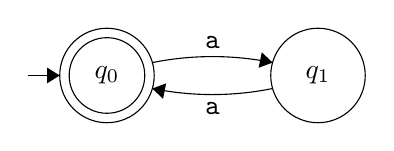
\begin{tikzpicture}[scale=0.2]
			\tikzstyle{every node}+=[inner sep=0pt]
			\draw [black] (31,-24) circle (3);
			\draw (31,-24) node {$q_0$};
			\draw [black] (31,-24) circle (2.4);
			\draw [black] (44.4,-24) circle (3);
			\draw (44.4,-24) node {$q_1$};
			\draw [black] (33.883,-23.181) arc (101.40687:78.59313:19.3);
			\fill [black] (41.52,-23.18) -- (40.83,-22.53) -- (40.63,-23.51);
			\draw (37.7,-22.3) node [above] {$\texttt{a}$};
			\draw [black] (26,-24) -- (28,-24);
			\fill [black] (28,-24) -- (27.2,-23.5) -- (27.2,-24.5);
			\draw [black] (41.52,-24.827) arc (-78.47234:-101.52766:19.113);
			\fill [black] (33.88,-24.83) -- (34.56,-25.48) -- (34.76,-24.5);
			\draw (37.7,-25.71) node [below] {$\texttt{a}$};
			\end{tikzpicture}
		\end{center}
		The circles represent the states and accepting states are denoted with a second inner circle. The arrows represent transitions and the labels are the symbols that need to be read for this transition to occur. The smaller arrow with no label designates the starting state.
		
		It is easy to see that the language recognized by this DFA consists of all the words with an even number of \texttt{a}'s (i.e.: $L(M) = \{\texttt{a}^{2n}: n \in \N\}$).
		
		\item The DFA recognizing the language $\{\texttt{a}^n\texttt{b}^m \mid n,m \in \N\}$ can be described as follows.
		\begin{center}
			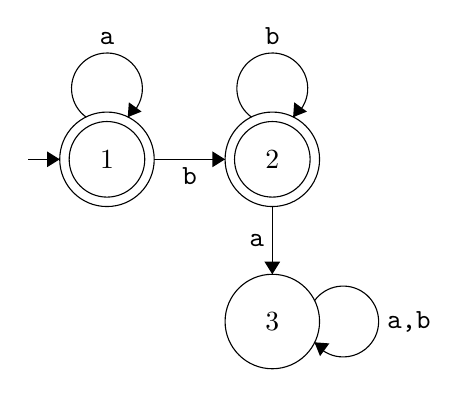
\begin{tikzpicture}[scale=0.2]
			\tikzstyle{every node}+=[inner sep=0pt]
			\draw [black] (5.1,-10.5) circle (3);
			\draw (5.1,-10.5) node {$1$};
			\draw [black] (5.1,-10.5) circle (2.4);
			\draw [black] (0.1, -10.5) -- (2.1, -10.5);
			\fill [black] (2.1, -10.5) -- (1.3,-10) -- (1.3,-11);
			\draw [black] (15.6,-10.5) circle (3);
			\draw (15.6,-10.5) node {$2$};
			\draw [black] (15.6,-10.5) circle (2.4);
			\draw [black] (15.6,-20.8) circle (3);
			\draw (15.6,-20.8) node {$3$};
			\draw [black] (8.1,-10.5) -- (12.6,-10.5);
			\fill [black] (12.6,-10.5) -- (11.8,-10) -- (11.8,-11);
			\draw (10.35,-11) node [below] {\texttt{b}};
			\draw [black] (14.277,-7.82) arc (234:-54:2.25);
			\draw (15.6,-3.25) node [above] {\texttt{b}};
			\fill [black] (16.92,-7.82) -- (17.8,-7.47) -- (16.99,-6.88);
			\draw [black] (18.28,-19.477) arc (144:-144:2.25);
			\draw (22.85,-20.8) node [right] {\texttt{a,b}};
			\fill [black] (18.28,-22.12) -- (18.63,-23) -- (19.22,-22.19);
			\draw [black] (3.777,-7.82) arc (234:-54:2.25);
			\draw (5.1,-3.25) node [above] {\texttt{a}};
			\fill [black] (6.42,-7.82) -- (7.3,-7.47) -- (6.49,-6.88);
			\draw [black] (15.6,-13.5) -- (15.6,-17.8);
			\fill [black] (15.6,-17.8) -- (16.1,-17) -- (15.1,-17);
			\draw (15.1,-15.65) node [left] {\texttt{a}};
			\end{tikzpicture}
		\end{center}
		\item For any DFA $M$ on an alphabet $\Sigma$, it is very easy to describe a DFA $M'$ that recognizes the complement of $L(M)$, i.e.: such that $L(M') = \Sigma^*\setminus L(M)$. We just invert the roles of accepting and non-accepting states. Here is the DFA recognizing the complement of $\{\texttt{a}^n\texttt{b}^m \mid n,m \in \N\}$.
		\begin{center}
			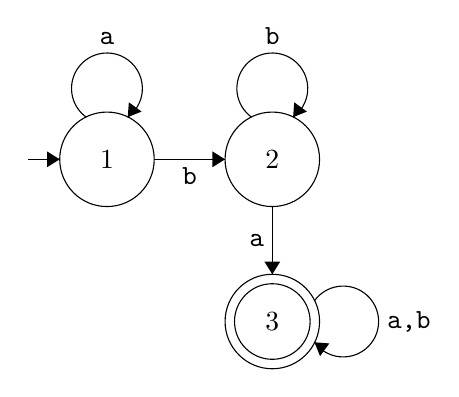
\begin{tikzpicture}[scale=0.2]
			\tikzstyle{every node}+=[inner sep=0pt]
			\draw [black] (5.1,-10.5) circle (3);
			\draw (5.1,-10.5) node {$1$};
			\draw [black] (0.1, -10.5) -- (2.1, -10.5);
			\fill [black] (2.1, -10.5) -- (1.3,-10) -- (1.3,-11);
			\draw [black] (15.6,-10.5) circle (3);
			\draw (15.6,-10.5) node {$2$};
			\draw [black] (15.6,-20.8) circle (3);
			\draw (15.6,-20.8) node {$3$};
			\draw [black] (15.6,-20.8) circle (2.4);
			\draw [black] (8.1,-10.5) -- (12.6,-10.5);
			\fill [black] (12.6,-10.5) -- (11.8,-10) -- (11.8,-11);
			\draw (10.35,-11) node [below] {\texttt{b}};
			\draw [black] (14.277,-7.82) arc (234:-54:2.25);
			\draw (15.6,-3.25) node [above] {\texttt{b}};
			\fill [black] (16.92,-7.82) -- (17.8,-7.47) -- (16.99,-6.88);
			\draw [black] (18.28,-19.477) arc (144:-144:2.25);
			\draw (22.85,-20.8) node [right] {\texttt{a,b}};
			\fill [black] (18.28,-22.12) -- (18.63,-23) -- (19.22,-22.19);
			\draw [black] (3.777,-7.82) arc (234:-54:2.25);
			\draw (5.1,-3.25) node [above] {\texttt{a}};
			\fill [black] (6.42,-7.82) -- (7.3,-7.47) -- (6.49,-6.88);
			\draw [black] (15.6,-13.5) -- (15.6,-17.8);
			\fill [black] (15.6,-17.8) -- (16.1,-17) -- (15.1,-17);
			\draw (15.1,-15.65) node [left] {\texttt{a}};
			\end{tikzpicture}
		\end{center}
	\end{enumerate}
\end{exmps}

\begin{rem}
    The term \textbf{deterministic} means that the transitions are completely determined by the input, that is, you can run the DFA on the same input many many times and it will always end in the same state and output the same thing. Mathematically, determinism comes from the fact that $\delta(q,a)$ takes the value of only one state for any $q \in Q$ and $a \in \Sigma$. If we allow $\delta$ to be nondeterministic, we get the definition of an NFA.
\end{rem}

\subsection{Nondeterminisitic Finite Automata}

\begin{defn}
	An \textbf{nondeterministic automaton} (NFA) $M$ consists of a finite alphabet $\Sigma$, a finite set of states $Q$ with a starting state identified by $q_0$, a transition function $\delta : Q \times (\Sigma \cup \{\varepsilon\}) \rightarrow \mP(Q)$ and a subset $F \subseteq Q$ of accepting states.
	
	There are two main differences with a DFA. First, an NFA can sometimes make a transition without reading a symbol from the input but rather by reading $\varepsilon$ (denoting an empty string). Second, the image of $\delta$ is a set of possible states for the transition to end in. Let us see how this affects the behavior of $M$.
	
	The automaton still reads its input letter by letter starting in state $q_0$, but now instead of making the only possible transition, it makes all of them at the same time and continues the computation on multiple branches. The output of $M$ is ``Accept'' if in at least one branch, all the input was read and $M$ is in an accepting state, otherwise $M$ outputs ``Reject''. The language recognized by $M$ is defined as for DFAs.
	
	Another way to view nondeterminism is to consider that $M$ has access to an all-knowing oracle that will choose which transition to make (out of the possible ones). This oracle always make the choices that lead to accepting the input if possible, hence, $M$ accepts $w \in \Sigma^*$ if and only if there is a sequence of choices that lead to an accepting state after reading all the input.
\end{defn}
\begin{exmps}
	The representation of NFAs is really similar to that of DFAs but now, arrows can be labeled with an $\varepsilon$, multiple arrows coming out of the same state can have the same label, and states can have no arrows coming out with a specific label $a \in \Sigma$ (corresponding to the fact that $\delta(q,\texttt{a}) = \emptyset$).
	\begin{enumerate}
		\item The NFA recognizing $\{\texttt{a}^n\texttt{b}^m \mid n,m \in \N\}$ is simpler than the DFA we drew above.
		\begin{center}
			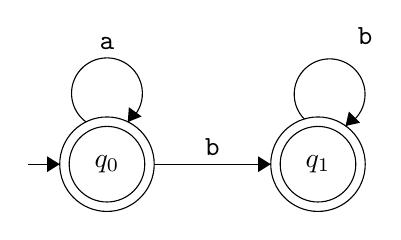
\begin{tikzpicture}[scale=0.2]
			\tikzstyle{every node}+=[inner sep=0pt]
			\draw [black] (31,-24) circle (3);
			\draw (31,-24) node {$q_0$};
			\draw [black] (31,-24) circle (2.4);
			\draw [black] (44.4,-24) circle (3);
			\draw (44.4,-24) node {$q_1$};
			\draw [black] (44.4,-24) circle (2.4);
			\draw [black] (34,-24) -- (41.4,-24);
			\fill [black] (41.4,-24) -- (40.6,-23.5) -- (40.6,-24.5);
			\draw (37.7,-23.5) node [above] {$\texttt{b}$};
			\draw [black] (26,-24) -- (28,-24);
			\fill [black] (28,-24) -- (27.2,-23.5) -- (27.2,-24.5);
			\draw [black] (29.677,-21.32) arc (234:-54:2.25);
			\draw (31,-16.75) node [above] {$\texttt{a}$};
			\fill [black] (32.32,-21.32) -- (33.2,-20.97) -- (32.39,-20.38);
			\draw [black] (43.536,-21.139) arc (224.53768:-63.46232:2.25);
			\draw (47.39,-16.44) node [above] {$\texttt{b}$};
			\fill [black] (46.15,-21.57) -- (47.07,-21.37) -- (46.36,-20.66);
			\end{tikzpicture}
		\end{center}
		\item For any DFA $M$, we can easily construct an NFA $M'$ that recognizes the reverse of $L(M)$, i.e.: $L(M') = \{w^{\mathcal{R}} \mid w \in L(M)\}$, where ${}^{\mathcal{R}}$ denotes the reverse of a word. Indeed, from the representation of a DFA, we can reverse all arrows, make the initial state an accepting state and add a pseudo initial state with $\varepsilon$--transitions to all the old accepting states as shown by the illustration below.
		
		The reverse of $\{\texttt{a}^n\texttt{b}^m \mid n,m \in \N\}$ is $\{\texttt{b}^n\texttt{a}^m \mid n,m \in \N\}$ and it is recognized by the following NFA.
	\begin{center}
		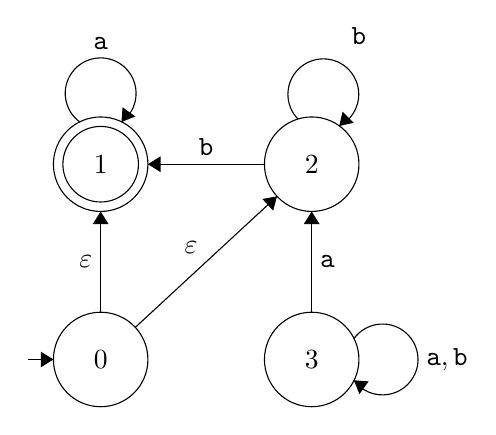
\begin{tikzpicture}[scale=0.2]
		\tikzstyle{every node}+=[inner sep=0pt]
		\draw [black] (31,-24) circle (3);
		\draw (31,-24) node {$1$};
		\draw [black] (31,-24) circle (2.4);
		\draw [black] (44.4,-24) circle (3);
		\draw (44.4,-24) node {$2$};
		\draw [black] (44.4,-36.4) circle (3);
		\draw (44.4,-36.4) node {$3$};
		\draw [black] (31,-36.4) circle (3);
		\draw (31,-36.4) node {$0$};
		\draw [black] (29.677,-21.32) arc (234:-54:2.25);
		\draw (31,-16.75) node [above] {$\texttt{a}$};
		\fill [black] (32.32,-21.32) -- (33.2,-20.97) -- (32.39,-20.38);
		\draw [black] (43.536,-21.139) arc (224.53768:-63.46232:2.25);
		\draw (47.39,-16.44) node [above] {$\texttt{b}$};
		\fill [black] (46.15,-21.57) -- (47.07,-21.37) -- (46.36,-20.66);
		\draw [black] (47.08,-35.077) arc (144:-144:2.25);
		\draw (51.65,-36.4) node [right] {$\texttt{a},\texttt{b}$};
		\fill [black] (47.08,-37.72) -- (47.43,-38.6) -- (48.02,-37.79);
		\draw [black] (44.4,-33.4) -- (44.4,-27);
		\fill [black] (44.4,-27) -- (43.9,-27.8) -- (44.9,-27.8);
		\draw (44.9,-30.2) node [right] {$\texttt{a}$};
		\draw [black] (41.4,-24) -- (34,-24);
		\fill [black] (34,-24) -- (34.8,-24.5) -- (34.8,-23.5);
		\draw (37.7,-23.5) node [above] {$\texttt{b}$};
		\draw [black] (26.4,-36.4) -- (28,-36.4);
		\fill [black] (28,-36.4) -- (27.2,-35.9) -- (27.2,-36.9);
		\draw [black] (31,-33.4) -- (31,-27);
		\fill [black] (31,-27) -- (30.5,-27.8) -- (31.5,-27.8);
		\draw (30.5,-30.2) node [left] {$\varepsilon$};
		\draw [black] (33.2,-34.36) -- (42.2,-26.04);
		\fill [black] (42.2,-26.04) -- (41.27,-26.21) -- (41.95,-26.95);
		\draw (36.74,-29.71) node [above] {$\varepsilon$};
		\end{tikzpicture}
	\end{center}
	
		\item Finding the complement of an NFA is not as easy as for DFAs. For instance, consider the following NFA on the alphabet $\{\texttt{a}, \texttt{b}\}$.
			\begin{center}
			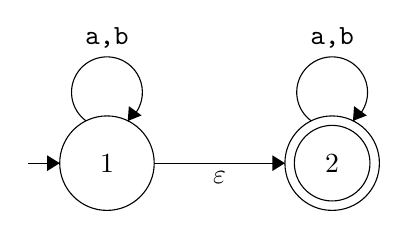
\begin{tikzpicture}[scale=0.2]
			\tikzstyle{every node}+=[inner sep=0pt]
			\draw [black] (5.1,-10.5) circle (3);
			\draw (5.1,-10.5) node {$1$};
			\draw [black] (0.1, -10.5) -- (2.1, -10.5);
			\fill [black] (2.1, -10.5) -- (1.3,-10) -- (1.3,-11);
			\draw [black] (19.4,-10.5) circle (3);
			\draw (19.4,-10.5) node {$2$};
			\draw [black] (19.4,-10.5) circle (2.4);
			\draw [black] (8.1,-10.5) -- (16.4,-10.5);
			\fill [black] (16.4,-10.5) -- (15.6,-10) -- (15.6,-11);
			\draw (12.25,-11) node [below] {$\varepsilon$};
			\draw [black] (18.077,-7.82) arc (234:-54:2.25);
			\draw (19.4,-3.25) node [above] {\texttt{a,b}};
			\fill [black] (20.72,-7.82) -- (21.6,-7.47) -- (20.79,-6.88);
			\draw [black] (3.777,-7.82) arc (234:-54:2.25);
			\draw (5.1,-3.25) node [above] {\texttt{a,b}};
			\fill [black] (6.42,-7.82) -- (7.3,-7.47) -- (6.49,-6.88);
			\end{tikzpicture}
		\end{center}
		It recognizes all words generated by the alphabet, but if you swap the accepting and non-accepting states, the new NFA will also accept all words.
	\end{enumerate}
\end{exmps}

\begin{rem}
    Since an NFA can have $\varepsilon$--transitions, the extension of $\delta$ to $\Sigma^*$ is defined differently, $\delta^*(x,\varepsilon)$ is the $\varepsilon$--\textbf{closure} of $x$ and $\delta^*(x,w)$ is defined inductively. More formally,
    \begin{align*}
        \delta^*(x,\varepsilon) &= \left\{q \in Q: \exists \{x= x_0, x_2, \dots, x_n = q\}, \forall 1\leq i \leq n, x_i \in \delta(x_{i-1}, \varepsilon) \right\}\\
        \delta^*(x, a\cdot w) &= \bigcup_{q \in \delta(x,a)} \bigcup_{q' \in \delta^*(q,w)} \delta^*(q', \varepsilon). 
    \end{align*}
    Intuitively, $\delta^*(x,w)$ is the set of words that $x$ can reach while reading the input $w$, taking into account that the machine can take any $\varepsilon$--transition.
\end{rem}

One question that quickly arises is whether there are languages that can be recognized by an NFA, but not by any DFA. The converse is clearly false because any DFA can be written as an NFA where the image of the transition function only contains singletons, i.e.: there is only one possible state for each transition.

Surprisingly, the original question also has a negative answer. In other words, any NFA has a DFA recognizing the same language. To prove this, we describe the powerset construction transforming an NFA into an equivalent DFA.

\begin{proof}[Proof sketch]
	Let $M = (\Sigma, Q, q_0, \delta, F)$ be an NFA, we construct an equivalent DFA $M' = (\Sigma, Q', q'_0, \delta', F')$ as follows.
	\begin{itemize}
		\item The states of $M'$ are sets of states of $M$, that is $Q' = \mP(Q)$.
		\item The initial state $q'_0$ is the set of states that can be reached by reading no symbol when running $M$. Formally, we have 
		\[q'_0 = \delta^*(q_0, \varepsilon).\]
		\item The transition function will simulate all the possible choices by transitioning between sets of states. For any $S \subseteq Q$ and $a \in \Sigma$,
		\[\delta'(S, a) = \bigcup_{q \in S} \delta^*(q,a)\]
		\item A set of states is accepting if and only if it contains an accepting state. 
	\end{itemize}
	It is left to show that $L(M) = L(M')$.
\end{proof}

The transformation we just described implies that NFAs are not necessary and we could always work with DFAs. However, observe that the size of the automaton increases exponentially in this procedure, so it is not practical to work with the resulting DFA. Consequently, one could ask whether we could further transform the DFA into a smaller (maybe smallest) but equivalent DFA. This is called DFA minimization and there are several polynomial time algorithms that solve this problem (Hopcroft's and Moore's). Another algorithm by Brzozowski is conceptually much simpler although it runs in exponential time in the worst case.
\subsection{Brzozowski's Algorithm}\label{sec-brzozowski}
\begin{defn}\label{defn-brzozowski}
    Let $M$ be a DFA, \textbf{Brzozowski's algorithm} is the following procedure.
    \begin{enumerate}
        \item Reverse $M$ to obtain an NFA $M^{\mathcal{R}}$ which recognizes the reverse of $L(M)$.
        \item Use the powerset construction to obtain a DFA $D(M^{\mathcal{R}})$, still recognizing the reverse of $L(M)$.
        \item Discard all unreachable states of $D(M^{\mathcal{R}})$, denote the automaton obtained with $N$.
        \item Apply the same procedure (steps 1 to 3) to $N$, i.e.: reverse $N$, determinize the result and discard unreachable states to obtain $O$. 
    \end{enumerate}
\end{defn}
\begin{prop}
    The final automata $O$ is the automaton with the least number of states satisfying $L(O) = L(M)$. Another way to say this: if $\textsf{rev}$ denotes the reversing operation, $\textsf{det}$ denotes the determinization and $\textsf{reach}$ denotes the operation of removing unreachable states, then \[\textsf{reach}(\textsf{det}(\textsf{rev}(\textsf{reach}(\textsf{det}(\textsf{rev}(M))))))\] is the minimal automaton equivalent to $M$.
\end{prop}
\begin{rem}
    This result should be very surprising. Brzozowski's algorithm simply reverses the automaton twice to obtain a minimal form. Moreover, during the procedure, there are two steps inducing an exponential blow-up of the number of states. Indeed, determinization via the powerset construction leads to an automaton with $2^{|Q|}$ states. That means that in the worst cases, $\textsf{det}(\textsf{rev}(\textsf{reach}(\textsf{det}(\textsf{rev}(M)))))$ could have $2^{2^{|Q|}}$ states. This is the reason why Brzozowski's algorithm can take exponential time. Nonetheless, in the end, you still end up with a minimal automaton. Another surprising thing, this algorithm often performs better than the worst case scenario.
\end{rem}
This algorithm was first proven correct using complex combinatorial arguments in 1963, but in this assignment, we will give a much simpler proof using coalgebras. The next section is dedicated to introducing coalgebras and coinduction via their duals, algebras and induction.

\section{Brzozowski's Algorithm Coalgebraically}
In this section we follow the proof given in \href{https://dl.acm.org/doi/10.1145/2490818}{this paper} (answers are in there). 
\subsection{Reachability and Observability}
Let $A$ be an alphabet, and $(X, i, \delta, F)$ be deterministic automaton, where $X$ is the set of states, $\delta:X \times A \rightarrow X$ is the transition function, $i \in X$ is the initial state and $F$ is the set of accepting states. For our purposes, we will view $i$ as a function $i: \mathbf{1} \rightarrow X$, $F$ as a function $f: X \rightarrow 2 = \{0,1\}$ and $\delta$ will also denote the curried version $\delta: X \rightarrow X^A$. This leads to the following simple representation of the automaton.

\begin{equation}\label{diag-dfa}
	\begin{tikzcd}
 \mathbf{1} \arrow[rd, "i"] & & 2 \\
 & X \arrow[d, "\delta"] \arrow[ru, "f"] & \\
 & X^A & 
 \end{tikzcd}
\end{equation}
In the light of the previous sections, we decompose this automaton into an algebra and a coalgebra.

First, we have the algebra $[i,\delta]: \mathbf{1}+(A\times X) \rightarrow X$ for the functor $\mathbf{1}+A\times (-)$. Recall from Exercise \ref{exer-initAlg} that $(A^*, [\textsf{nil}:=\varepsilon, \textsf{cons}])$ is initial for the functor $1+(A\times -)$, so after currying $\textsf{cons}$, we obtain a unique morphism $r:A^*\rightarrow X$ that makes the following diagram commute.
\begin{equation}\label{diag-dfainit}
    \begin{tikzcd}
        \mathbf{1} \arrow[rd, "i"] \arrow[d, "\varepsilon"']  &                                       & 2 \\
        A^* \arrow[d, "\textsf{cons}"'] \arrow[r, "r", dashed] & X \arrow[d, "\delta"] \arrow[ru, "f"] &   \\
        (A^*)^A \arrow[r, "r^A"', dashed]                      & X^A                                   &  
        \end{tikzcd}
\end{equation}
Explicitly, the commutativity of the left half of diagram \ref{diag-dfainit} amounts to
\[
r(\varepsilon) = i \quad \text{ and } \quad 
r(\textsf{cons}(w,a)) = \delta(r(w),(a)), \forall a \in A
\]
We infer that for any word $w \in A^*$, $r(w)$ is the state reached by the automaton after starting in state $i$ and reading input $w$.

Second, we have the coalgebra $(f,\delta): X \rightarrow 2 \times X^{A}$. Recall from diagram \ref{diag-finalcoalgexmp} that $(2^{A^*}, (\varepsilon?, \omega))$ is final for the functor $2\times (-)^A$. Thus, we obtain a unique morphism $o:X \rightarrow 2^{A^*}$ that completes diagram \ref{diag-dfainit}.
\begin{equation}\label{diag-dfainitfinal}
	\begin{tikzcd}
 \mathbf{1} \arrow[rd, "i"] \arrow[d, "\textsf{nil}"'] & & 2 \\
 A^* \arrow[d, "\textsf{cons}"'] \arrow[r, "r", dashed] & X \arrow[d, "\delta"] \arrow[ru, "f"] \arrow[r, "o", dashed] & 2^{A^*} \arrow[u, "\varepsilon?"'] \arrow[d, "\omega"] \\
 (A^*)^A \arrow[r, "r^A"', dashed] & X^A \arrow[r, "o^A"', dashed] & (2^{A^*})^A 
 \end{tikzcd}
\end{equation}

We recall from Exercise \ref{exer-finalcoalg} that for any $x \in X$, $o(x)$ is the language in accepted by the automaton if started on state $x$.

\begin{defn}
	In the setting above, the automaton $(X,i, \delta,f)$ is said to be
	\begin{enumerate}
		\item \textbf{reachable} if $r$ is surjective,
		\item \textbf{observable} if $o$ is injective, and
		\item \textbf{minimal} if it is both reachable and observable.
	\end{enumerate}
\end{defn}
\begin{exer}[1pts]
    \begin{enumerate}[(a)]
        \item Describe, in automata theoretic terms, what reachability and observability mean.
        \item Informally explain why an automaton has a minimal number of states if and only if it is both reachable and observable.
    \end{enumerate}
\end{exer}

\subsection{Reversing an Automaton}
We will use our new method of representing automata to give the construction of an automata which recognizes the reverse language. Morally, our procedure does the same thing as the original reversing algorithm and the powerset construction at the same time.

In the sequel, let $2^{(-)}$ denote the contravariant powerset functor, namely, it sends $X$ to $2^X$ and $f: X \rightarrow Y$ to $2^f: 2^Y \rightarrow 2^X = S \mapsto \{x \in X: f(x) \in S\}$.

The reversed powerset construction goes like this. Given a transition function $\delta: X \rightarrow X^A$, we can uncurry it to get $\delta : X\times A \rightarrow X$, then apply $2^{(-)}$ to obtain $2^{\delta}: 2^X \rightarrow 2^{X\times A}$ and finally curry the elements in the codomain to obtain $2^{\delta}: 2^X \rightarrow (2^X)^A$. This is now a transition function for an automata whose states are set of states of the original automata.
\begin{exer}[3pts]
    \begin{enumerate}[(a)]
        \item Describe the action of $2^{\delta}$.
        \item Continue applying $2^{(-)}$ to the L.H.S. of diagram \eqref{diag-dfainitfinal} to obtain \eqref{diag-dfarev}. Briefly describe what each depicted morphism does.
        \begin{equation}\label{diag-dfarev}
            \begin{tikzcd}
            & 2 \\
            2^X \arrow[ru, "2^i"] \arrow[d, "2^{\delta}"'] \arrow[r, "2^r"] & 2^{A^*} \arrow[u, "2^{\textsf{nil}}"'] \arrow[d, "2^{\textsf{cons}}"] \\
            (2^X)^A \arrow[r, "2^{r^A}"'] & (2^{A^*})^A 
            \end{tikzcd}
        \end{equation}
        \textbf{Warning:} For $\textsf{cons}$, you will need to use the same trick as for $\delta$.
    \end{enumerate}
\end{exer}
By currying $f:X \rightarrow 2$ to $f: \mathbf{1} \rightarrow 2^X$, we obtain an $\mathbf{1}+ A\times(-)$-algebra structure on $2^X$ which, by initiality of $A^*$, gives the following diagram.
\begin{equation}\label{diag-dfarevall}
\begin{tikzcd}
\mathbf{1} \arrow[rd, "f"] \arrow[d, "\textsf{nil}"'] & & 2 \\
A^* \arrow[d, "\textsf{cons}"'] \arrow[r, "R", dashed] & 2^X \arrow[ru, "2^i"] \arrow[d, "2^{\delta}"'] \arrow[r, "2^r"] & 2^{A^*} \arrow[u, "2^{\textsf{nil}}"'] \arrow[d, "2^{\textsf{cons}}"] \\
(A^*)^A \arrow[r, "R^A"', dashed] & (2^X)^A \arrow[r, "2^{r^A}"'] & (2^{A^*})^A 
\end{tikzcd}
\end{equation}
This is very close to what we are looking for:
\begin{itemize}
    \item We have an automaton whose states are $2^X$,
    \item its initial state is the set of states which contain at least one final state of the original automaton,
    \item its final states are the set of states which contain the initial state of the original automaton, and
    \item the morphism $R$ tells us which states are reachable.
\end{itemize}
However, the R.H.S. of \eqref{diag-dfarevall} is not excatly what we need to talk about observability of this automaton. You can see that $2^{\textsf{nil}} = \varepsilon?$, but $2^{\textsf{cons}}$ is a kind of reversed version of $\omega$, the concatenation is done in the opposite way.
\begin{exer}[1pts]
    Describe the unique way to complete \eqref{diag-dfarevall} into \eqref{diag-dfacomplete}.
    \begin{equation}\label{diag-dfacomplete}
    \begin{tikzcd}
    \mathbf{1} \arrow[rd, "f"] \arrow[d, "\textsf{nil}"'] & & 2 \\
    A^* \arrow[d, "\textsf{cons}"'] \arrow[r, "R", dashed] & 2^X \arrow[ru, "2^i"] \arrow[d, "2^{\delta}"'] \arrow[r, "O", dashed] & 2^{A^*} \arrow[u, "\varepsilon?"'] \arrow[d, "\omega"] \\
    (A^*)^A \arrow[r, "R^A"', dashed] & (2^X)^A \arrow[r, "O^A"', dashed] & (2^{A^*})^A 
    \end{tikzcd}
    \end{equation}
\end{exer}
In conclusion, we have an automaton $(2^X, f, 2^{\delta}, 2^i)$ which is reachable if $R$ is surjective and observable if $O$ is injective. Moreover, we can show two imporant properties.

\begin{exer}[4pts]
    \begin{enumerate}[(a)]
        \item If $(X, i, \delta, f)$ recognizes the language $L$, then $(2^X, f, 2^{\delta}, 2^i)$ recognizes the reverse of $L$.
        \item If $(X, i, \delta, f)$ is reachable, then $(2^X, f, 2^{\delta}, 2^i)$ is observable.
    \end{enumerate}
\end{exer}

\subsection{Correctness of the Algorithm}
\begin{exer}[1pt]
    Show that Brzozowski's algorithm is correct. Namely, if $(X,i, \delta, f)$ recognizes a language $L$, then
    \begin{itemize}
        \item applying the (new) reverse construction, 
        \item keeping only the reachable states,
        \item applying the reverse construction again, and
        \item keeping only the reachable states
    \end{itemize}
    yields an automaton which is minimal and recognizes the language $L$.
\end{exer}
\end{document}